\documentclass{standalone}

\usepackage{tikz}
\usepackage{pgfplots}

\newcommand{\xa}[0]{0.34}
\newcommand{\xb}[0]{-0.2}
\newcommand{\xc}[0]{0.7}
\newcommand{\potential}[1]{2*(1-4*#1^2)^2+1.3*#1}

\usetikzlibrary{positioning, decorations}

\begin{document}
\begin{tikzpicture}
    \node at (0,0) (a1){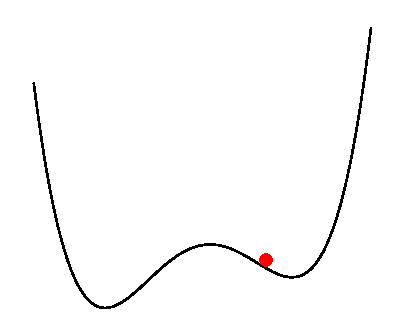
\includegraphics[width=0.2\textwidth]{pot1.pdf}};
    \node[below=0cm of a1](a2){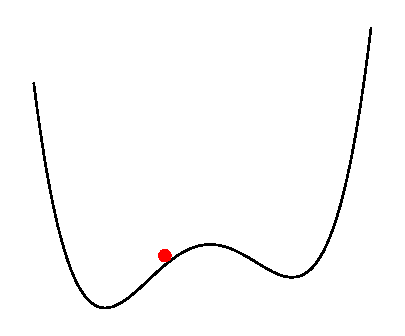
\includegraphics[width=0.2\textwidth]{pot2.pdf}};
    \node[below=1cm of a2](dots){$\vdots$};
    \node[below=1cm of dots](a3){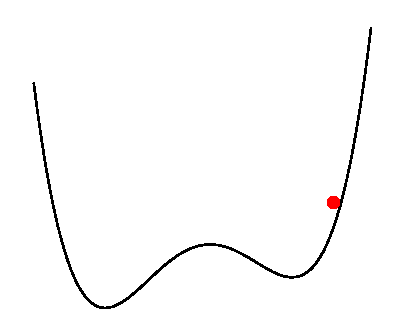
\includegraphics[width=0.2\textwidth]{pot3.pdf}};

    \draw[decorate, decoration=brace, thick](a1.north east) -- node[midway](bracemid){}(a3.south east);

    \node[right=2cm of bracemid](all){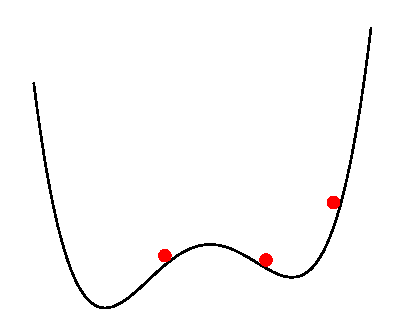
\includegraphics[width=0.2\textwidth]{allpot.pdf}};

    \draw[->, thick] (bracemid) -- (all);

    \node[above left=0cm and 0cm of a1]{(a)};
    \node[above left=0cm and 0cm of all]{(b)};
\end{tikzpicture}
\end{document}